\begin{figure}[H]
\centering
\resizebox{0.4\textwidth}{!}{
   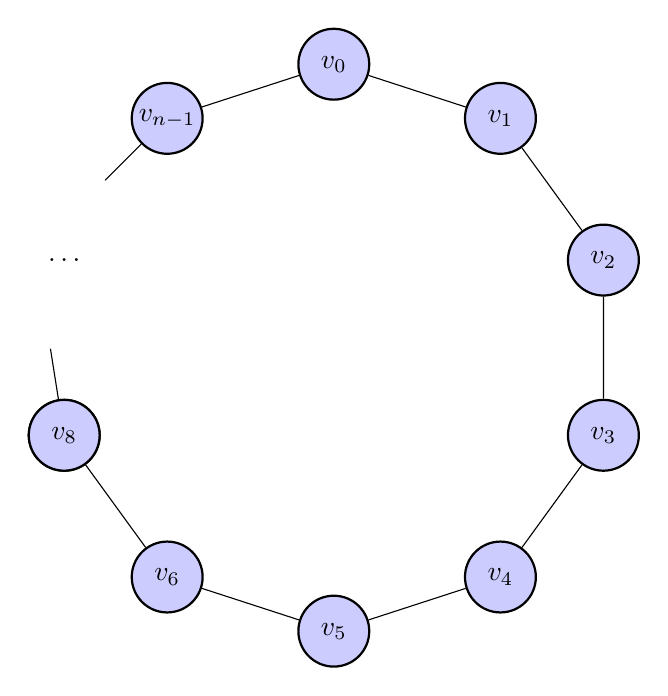
\begin{tikzpicture}[scale=1.2, auto=left, every node/.style={circle, fill=blue!20, draw=black, thick, inner sep=0pt, minimum size=0.9cm}]

     % Vértices visibles de v_0 a v_8 en sentido horario
     \node (v0) at (90:3) {$v_0$};
     \node (v1) at (54:3) {$v_1$};
     \node (v2) at (18:3) {$v_2$};
     \node (v3) at (-18:3) {$v_3$};
     \node (v4) at (-54:3) {$v_4$};
     \node (v5) at (-90:3) {$v_5$};
     \node (v6) at (-126:3) {$v_6$};
     \node (v7) at (-162:3) {$v_7$};
     \node (v8) at (198:3) {$v_8$};

     % Último vértice v_{n-1}
     \node (vn1) at (126:3) {$v_{n-1}$};

     % Vértices invisibles y puntos para la discontinuidad
     \node[draw=none, fill=none, minimum size=0pt] (v9_inv) at (180:3) {};
     \node[draw=none, fill=none, minimum size=0pt] (vn2_inv) at (144:3) {};
     \node[draw=none, fill=none, minimum size=0pt] (dots) at (162:3) {$\dots$};

     % Aristas continuas principales
     \draw (v0) -- (v1);
     \draw (v1) -- (v2);
     \draw (v2) -- (v3);
     \draw (v3) -- (v4);
     \draw (v4) -- (v5);
     \draw (v5) -- (v6);
     \draw (v6) -- (v7);
     \draw (v7) -- (v8);

     % Arista normal entre v_{n-1} y v_0
     \draw (vn1) -- (v0);

     % Aristas hacia/desde la zona discontinua
     \draw (v8) -- (v9_inv);
     \draw (vn2_inv) -- (vn1);

   \end{tikzpicture}}%
   \caption{El grafo $C^n$}
   \label{fig:ciclo_n}
\end{figure}
